%!TEX root = ../thesis.tex
%*******************************************************************************
%*********************************** First Chapter *****************************
%*******************************************************************************

\chapter{Introduction}  %Title of the First Chapter

\ifpdf
     \graphicspath{{Figs/Chapter1/}}
\else
    \graphicspath{{Chapter1/Figs/Vector/}{Chapter1/Figs/}}
\fi


%********************************** %First Section  **************************************

\section{Overview} %Section - 1.1 

\emph{"... as they say, your model is only as good as the data you have. \newline So it all starts with the data ..."} \newline
\indent \indent - Nyalleng Moorosi, \emph{Deep Learning Indaba} (2017) \par

\smallskip

\noindent Artificial intelligence (AI) is the imitation of human-level intelligence by machines. Human beings are capable of extracting information from a passage of text, and transforming that information into a mental model of objects and relationships between those objects. As stated by Nyalleng Moorosi, the model is only as good as the data data available for training, and this is true for both human mental models as well as machine constructed models. \par

\noindent Human models can be confined to a single domain \unskip~\citep{staab2010handbook}, for example the entertainment industry. The entertainment industry contains objects such as films, actors, actresses, characters and awards. These objects have relationships between them, such as "stared in", "worked along side", "a character in", and "was nominated for". Humans can develop a mental model to easily reason about new relationships between the objects that were not mentioned in a given passage of text. For example the text may say that Chadwick Boseman starred in a film called Black Panther and played the character Black Panther. Using that information we can reason that Chadwick Boseman "is an" actor. \par

\noindent We use such models to read and understand other passages of text, in conversations with other people, and to help us answer questions. The set of objects and the relationships between them, within a domain, can be thought of as knowledge. Figure 1.1. shows what knowledge about the entertainment industry might look like. 

\begin{figure} [H]
   	\centering
    	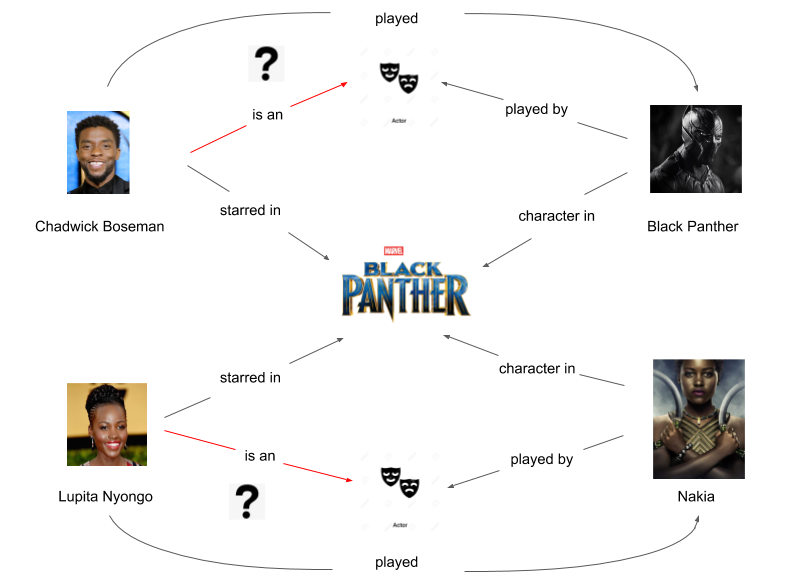
\includegraphics[width=0.8\textwidth, height=0.4\textheight]{Entities_and_the_Relationships_Between_Them}
	\captionsetup{justification=centering}
	\caption{Objects and relationships between them. We see Chadwick Boseman starred in the Black Panther film and played the Black Panther character. We also see that the character was played by an actor, and can reason that Chadwick Boseman may thus be an actor.}
\end{figure}

\subsection{Challenges} 

Reasoning about knowledge expressed in natural language \unskip~\citep{minervini2019differentiable} is simple for humans, but trying to imitate this behaviour on a computer reveals its underlying complexity. \par

\noindent The first task is providing a mechanism for perceiving syntax. Humans recognise text as sequences of words, and words as a sequence of characters. Characters can belong to different writing systems which can be dense (have a few characters used in a large number of combinations), or sparse (have a large number of characters used in fewer combinations) \unskip~\citep{Hua2010}. A computer has to first be able to perceive these characters. \par

\noindent The second task is even more challenging: modelling semantics. Semantics is the meaning of words in language \unskip~\citep{chomsky1955logical}. It allows humans to understand each other in conversation, through written text, and through visual imagery. Semantics allows us to understand that an actor is a thing, and that things can have relationships with other things. Giving computers the capability of semantic understanding is challenging because of the unstructuredness of language. If a person is shown a word in the singular and a word in the plural, for example "film" and "films", a person will most likely understand that there is not much difference in meaning between the two words, while a computer may interpret them as having completely different meanings. Different words can also have similar meanings, for example "film" and "movie". Capturing this similarity once again challenging for machines. And finally the order in which words are seen can provide context, for example the word "star" has completely different meanings in "Chadwick Boseman is a movie star" and "Black Panther looked up into the night sky and saw a star". \par

\noindent The third challenging task is organising information in such a way as to be able to reason about the knowledge it conveys. Humans build mental models using default reasoning \unskip~\citep{reiter1980logic}, believing that most objects A have some relationship X with objects B, with a small number of exceptions. For example, we could believe that films (object A) have not won (relationship X) an Oscar (object B). We will believe this is true for any given movie, unless we are familiar enough with movie history to identify the exceptions. Formallly, the default beliefs we hold are facts, and this process of reasoning allows us to infer new facts in the form of plausible relationships between objects. \par

\noindent In order to allow computers to use a similar method of reasoning, facts can be represented as graph-structured data. Such a representation is called a knowledge graph (KG) and models facts as entities (nodes) and the relations (edges) between them \unskip~\citep{nickel2015review}. The Resource Description formalism (RDF) is used to encode facts as triples in the form, subject-predicate-object, where the subject and object are entities, and the predicate is a relation between two entities \unskip~\citep{bizer2009dbpedia}. For example, a fact (triple) in an entertainment KG would be Black Panther (subject/entity) is a (predicate/relation) super hero (object/entity). \par

\noindent Question answering (QA) relies on knowledge discovery, the step-by-step deductive process used to infer possible facts given known facts. This is the process used above to infer that Chadwick Boseman is an actor, given other facts known about Chadwick Boseman and the Black Panther film. Statistical relational learning (SRL) solves the knowledge discovery problem by constructing models with measures of uncertainty in plausible facts not contained in KGs \unskip~\citep{koller2007introduction}.\par

\subsection{Encouraging progress} 

The task of QA can be extended to an open-domain setting \unskip~\citep{chen2017reading}, where the task is extended from answering questions from a single domain to a multiple domains. In this setting, a KG contains data from multiple domains and more complex knowledge discovery chains be constructed. There has been encouraging progress in SRL to modelling this problem, and link prediction is now often used as a paradigm for knowledge discovery \unskip~\citep{kristiadi2019incorporating, ebisu2018toruse, nguyen2017novel}. Latent feature modelling using tensor factorisation \unskip~\citep{harshman1978models, kolda2009tensor} is an approach to link prediction that has seen some promising results \unskip~\citep{bordes2011learning, jenatton2012latent, nickel2016holographic}. \par 

\noindent The first major milestone was demonstrating the bilinear tensor product as a promising model to link prediction \unskip~\citep{nickel2011three}. In this model, the multiplication is taken between a subject vector and a predicate matrix, producing a entity-relational vector. The dot product is then taken between the entity-relational vector and an object vector, which generates a relational score between the subject and object entities. \par

\noindent The second milestone was the integration of the bilinear tensor product and neural networks \unskip~\citep{socher2013reasoning}. In this approach a recursive network \unskip~\citep{pollack1990recursive} computes a compositional score between the subject and object, which is then added to a bilinear tensor product score. The result is then passed through a nonlinearity which generates the final relational score. This approach effectively extended linear tensor factorisation techniques to nonlinear techniques, and simultaneously introduced the use of pre-trained word embeddings to initialise entity and relation vectors instead of random initialisation. In this one approach both decision making expressiveness as well as entity and relation semantic representations were improved. \par

\noindent The third time a milestone was realised was with the use of complex valued embeddings for link prediction \unskip~\citep{trouillon2016complex}. This approach extended the bilinear tensor product by making use of the Hermitian dot product, which is the complex counterpart of the standard dot product between real vectors. It was proposed that complex vectors can effectively capture antisymmetric relations, "is not", while retaining the efficiency benefits of the dot product. This was achieved by using representations with complex embeddings, allowing the model to capture semantic meaning by computing a relational score dependent on the order of the entities in the triple. \par
 
\noindent The previous three milestones relied on shallow models that could scale to large datasets. Up until that point research in link prediction had focused on minimising the parameterisation of models. Convolutional networks are parameter efficient models, and major progress was again realised with the use of deep convolutional models for link prediction \unskip~\citep{dettmers2018convolutional}. The approach made use of 2D embedding representations which allowed the modelling of a large number of interactions between entities, achieving state-of-the-art (SOTA) link prediction performance as a result. \par

\subsection{Remaining challenges}

\noindent Open-domain knowledge graph question answering (KGQA) is getting closer to realising a form of AI reasoning generalisation. One significant challenge still faced by this framework is automatic construction of KGs \unskip~\citep{dong2014knowledge}. These large data sources are required to adequately train link prediction models. Combining such data sources for sufficient knowledge density remains an open area of research \unskip~\citep{diefenbach2018wdaqua}. Relying on systems with a graph structure alone limit the set of available resources which can be used to acquire knowledge \unskip~\citep{chen2017reading}, which necessitates the use of other source types including news document sets amongst others. Presenting this information poses a significant data transformation challenge, as well as potentially requiring continual online learning of the model as new data becomes available \unskip~\citep{abujabal2018never}. \par

\noindent It is also currently unclear which link prediction paradigm is the most useful in knowledge discovery. In addition to latent feature modelling, graph modelling \unskip~\citep{niepert2016discriminative, schlichtkrull2018modeling, pinter2018predicting} and inductive probabilistic logic programming (PLP) \unskip~\citep{yang2017differentiable, speichert2018learning} are two approaches also used for link prediction. Graph modelling is a generalisation of latent feature modelling which aggregates local and global entity neighbourhood context to generate relational scores between entities. Inductive PLP introduces stochastic primitives to logic programming languages. Recently graph modelling has been receiving increased attention as an approach to link prediction, and may reveal efficient knowledge discovery patterns. \par

\noindent Finally, there seems to be large headroom for improvement in latent feature modelling-based link prediction. SOTA performance on standard benchmark datasets, where the task of discovering the top 10 most plausible facts given an entity-relational composition, is currently achieved by a graph modelling technique \unskip~\citep{ruderNLPProg}. There is currently no human-level benchmark with which to contrast this performance, and it is also unclear whether improvement in link prediction performance can be realised by further optimisations to tensor factorisation approaches, or if a paradigm shift to graph modelling or inductive PLP will be required.  

\subsection{Outline of contributions}

SOTA neural factorisation models \unskip~\citep{balazevic2019hypernetwork, dettmers2018convolutional} introduce relational covariate shift \unskip~\citep{ioffe2015batch} - distortion of relational matrix parameters during training due to simultaneous updates of parameters in the previous layer. The models extend the bilinear model \unskip~\citep{jenatton2012latent}, a multiplicative linear compositional model, by computing subject-predicate transformations using a convolutional operation \unskip~\citep{zeiler2014visualizing}, instead of a dot product. This extension exacerbates covariate shift between the subject and predicate features. We correct for this exacerbated covariate shift by regularising relational filters using batch normalisation. \par

\noindent Leveraging semantic information \unskip~\citep{socher2013reasoning} from pre-trained word embeddings \unskip~\citep{mikolov2013distributed} can provide richer representations for improved inference during reasoning. We integrate pre-trained word embeddings into SOTA neural factorisation model training to compensate for this sparsity in representational data, providing richer context with which to perform reasoning. 

\subsection{Long-term motivations} 

Reasoning about knowledge expressed in natural language is one of the strongest measures of intelligence possessed by humans. This capability allows challenges discourse, debate and dialogue. In order for humans to realise artificial general intelligence (AGI), this skill has to be mastered by machines. Potential applications that can be designed using such technology have profound implications for all aspects of society, challenges including in education (such as tutoring system), health (such as frontline assistance), and science (from applications in astronomy to energy research). Practical implementations of AGI will likely be grounded in natural language and the internet. This thesis aims to contribute implementations that can help in methodology understanding toward the realisation of full AGI.  

\subsection{Short-term motivations}

We note the poor performance in open domain question answering i.e. inferring potential answers from know facts, currently achieved by SOTA neural factorisation models \unskip~\citep{balazevic2019hypernetwork, dettmers2018convolutional}. A sensible implementation of AGI would use heterogeneous information sources from the internet \unskip~\citep{angeli2013philosophers}. Extracting information from the web, constructing or expanding knowledge bases, and then answering questions \unskip~\citep{shalaby2019beyond} is currently the most successful paradigm for open domain question answering. Given that the most successful models using this paradigm have poor performance, there is an opportunity to refine existing techniques in an effort to make them more useful in answering questions in this way. Revolutionising existing methods that try to solve AI tasks by making use of deep learning techniques has seen tremendous progress in fields such as computer vision \unskip~\citep{hudson2018compositional}  and natural language processing \unskip~\citep{peters2018deep}. Neural factorisation approaches should attempt further integration of deep learning methods, with the adoption of practices from such fields applied to training, reasoning and knowledge representation. Given that deep learning itself is loosely modelled after the human mind, it seems sensible to try to bring SRL into closer alignment with methods of reasoning used by humans. 

\subsection{Challenges of tensor factorisation} 

In order to answer open-domain questions, the domain in which the knowledge belongs needs to be defined. Facts about that domain then need to be populated. Typically this is achieved by scanning documents written in natural language on the internet \unskip~\citep{fader2011identifying, dong2014knowledge} and populating a knowledge base. Given the heterogeneity of these data sources, it can be difficult to consolidate the information into a central datastore which can then be used to perform inference.  Related to the problem of centralising knowledge, the number of facts within a domain can range from hundreds of thousands, to millions. This poses a sample scarcity or model density problem. In the former, it becomes a challenge to adequately model the probability distributions of plausible relations given the frequency in observations of facts about a particular subject. In the latter, large parameterisation of models is needed to encode knowledge within the domain. \par

\noindent An additional challenge to this method of question answering is the compute resources required to perform inference. For any given question, current methods perform an inference test on every entity within the knowledge base. This is not a challenge for knowledge bases with a small number of entities, for example tens of thousands of entities, however it poses a serious scalability problem for knowledge bases with entities in the millions. This compute problem presents significant opportunity for more scalable inference implementations. Similarly, question answering is modelled as a classification task, where the classification categories are the entities themselves. This means large numbers of target categories are in the millions, whilst small numbers of target categories are in the tens of thousands. This seems like an impractical method of modelling question answering and also presents opportunity for improvement. 


%********************************** %Second Section  *************************************

\section{Related work} %Section - 1.2 

\subsection{Reasoning about facts} 

\noindent This thesis aims to extend research that aspires to give computers the capability of human-like reasoning \unskip~\citep{bordes2011learning} in open domain question answering \unskip~\citep{hakimov2019evaluating}. Early work in this area focused on learning deterministic logical concepts based on symbolic frameworks \unskip~\citep{hohenecker2017deep} which were used for formal reasoning. Later, attempts to relax formal reasoning and make use of more flexible embedding representations of natural language inspired research in SRL \unskip~\citep{koller2007introduction}. Link prediction is an SRL approach to human-like reasoning that makes use of knowledge bases \unskip~\citep{balazevic2019hypernetwork, dettmers2018convolutional, socher2013reasoning}. \par

\noindent Early approaches to reasoning over facts in KBs were attempted using tensor factorisation \unskip~\citep{nickel2011three} to model entity-relational interactions. Nickel et al. implemented RESCAL, a model that uses the bilinear tensor product to model interactions where entities are expressed as vectors and and the relation between them is represented as a full rank matrix \unskip~\citep{nickel2012factorizing}. The triple is then scored by computing the product of pairwise interactions between latent features of the respective representations \unskip~\citep{nickel2015review} and producing a measure of confidence in the fact. RESCAL uses the values of the relational matrix to model block structure patterns (groups of entities that have similar relationships to other groups), homophily patterns (the tendency of entities to be related to other entities with similar characteristics), and anticorrelations (the tendency of entities with different characteristics to produce antirelations). \par

\noindent Translating the embeddings (TransE) of entities by Bordes et al. \unskip~\citep{bordes2013translating} was another approach tried to model entity-relational interactions. The motivation for this approach was that a lot of KB facts are presented in hierarchies, therefore a translation of the subject by the predication should produce an embedding close to the object. The model translation is thus the natural transformation of the entity and can be used to model hierarchies, along with embedding equivalence with the null transformation. \par

\noindent Yang et al. proposed DistMult \unskip~\citep{yang2014embedding}, a bilinear diagonal model which first transforms the subject and object entities into low-dimensional vector representations, and then applies a bilinear tensor product operation using a relation matrix with only diagonal elements. This approach effectively models a subset of the entity-relational interactions of RESCAL and relies on the entity transformations to generate sufficient semantic representations. The model's bilinear formulation is extremely parameter efficient, but lacks expressiveness. \par

\noindent ComplEx \unskip~\citep{trouillon2016complex} by Trouillon et al. is the extension of DistMult into the complex domain. Entities are represented using complex vectors, and relations are represented using a diagonal matrix with complex entries. Complex valued embeddings extend the modelling of entity-relational interactions to include antisymmetric interactions. \par

\noindent All these approaches rely on linear composite triple representations - the multiplicative operator on the subject vector and relation matrix, followed by the dot product of the generated representation and object vector. These representations scale well with large datasets but are limited in their expressiveness. Next we will discuss nonlinear composite triple representations. \par

\noindent Neural tensor networks (NTN) were proposed by Socher and Chen et al. \unskip~\citep{socher2013reasoning}. NTNs approach link prediction by extending the bilinear tensor product in two ways. Firstly, they model interactions between subject and object entities using a recursive neural network (RCNN) \unskip~\citep{socher2012semantic}, which model constructs a representation that is added to the bilinear tensor product. Secondly, the resultant representation is passed through a neural network. The NTN thus expresses richer semantic information by using the RCNN, and increases the expressiveness of entity-relational interactions using a neural triple representation composition. Socher and Chen also examine the use of pre-trained word embeddings on link prediction. They find that models trained using word embeddings outperform models trained using random initialisation. \par

\noindent Hohenecker and Lukasiewicz extended NTNs by pre-computing object representations as aggregations of all the triples in which the object plays a part \unskip~\citep{hohenecker2017deep}. They introduce the new model as a relational NTN (RTN). Dong et al. introduced ER-MLP \unskip~\citep{dong2014knowledge, nickel2015review}; a simplification of NTN. This model extends the entity-relational interaction model by passing the bilinear tensor product through a neural network. ER-MLP also makes use of low-dimensional vectors for word embedding representations. \par

\noindent HolE, by Nicel et al., uses a  circular correlation to create compositional representations \unskip~\citep{nickel2016holographic}. It relies on a concatenation of the subject and object entities, directly modelling the relational score on shared semantic features of the entities. The relational vector is then used to project the representation, before a sigmoidal nonlinearity is used to complete the composition and score the relation. This approach is particularly adept at modelling anti-symmetric interactions. HolE introduces the concept of dynamically training embeddings to represent observed relations instead of storing static entity and relation embeddings. \par

\noindent Dettmers et al. introduced ConvE \unskip~\citep{dettmers2018convolutional}. ConvE provides a more expressive model by taking the convolution of triple entities with a 2-dimensional convolutional relational model. The subject vector and the relation vector are each reshaped into a matrix and lengthwise concatinated. A convolution operation is then performed on the matrices where the relation matrix performs the task of the relational filter. The obtained feature maps are then flattened and put through a fully connected layer. Finally, the inner product of the generated representation is taken with all object entity vectors to generate a score for each triple. ConvE  increases expressiveness by modelling entity-relational interactions  around the entire concatenation line, therefore modelling additional points of interaction between embeddings. \par

\noindent The above modelling approaches form part of latent feature modelling in link prediction. Two other research categories, namely graph modelling and inductive probabilistic logic programming, represent additional attempts at link prediction. We refer the reader to \unskip~\citep{nickel2015review} for a recent review of such approaches. \par

\subsection{Entity and relation representations} 

\noindent Previous work represented entities and relations using randomly initialised, static vector representations. This approach does not allow the sharing of statistical strength between the words describing each entity \unskip~\citep{socher2013reasoning}. Socher and Chen et el. showed that using pre-trained word embeddings instead of randomly initialised word embeddings improves link prediction model performance. This performance gain can be explained by the co-occurrence statistics used to train word embeddings. The semantic and syntactic similarity between words captured by word embeddings helps identify plausible interactions between entities. For example, we would expect film and character entities to be collocated in pre-trained embeddings spaces. The following describes approaches used to generate such embeddings. \par

\noindent Word2Vec, introduced by Mikolov et al., is an algorithm for training distributed representations of words \unskip~\citep{mikolov2013distributed}. The skip-gram model ~\citep{mikolov2013efficient} is one of the models used by Word2Vec to generate word vectors from very large text corpora (more than a billion words). The model essentially takes a centre word, and then tries to predict the probability of seeing a context word to the right or left of the centre word. This context window also be longer than one word. The skip-gram model uses the hierarchical softmax loss function \unskip~\citep{morin2005hierarchical} for classification (a computationally efficient approximation of the full softmax) and employs the subsampling of frequent stop words such as “in”, “the”, and “a”. The continuous bag of words (CBOW) \unskip~\citep{mikolov2013efficient} is an alternative approach to the skip-gram model. Here the model tries to predict a target word, given a sequence of context words. The CBOW has the advantage of being faster to train and producing better representations for more frequent words. \par

\noindent GloVe, by Pennington et al., is another unsupervised learning algorithm for generating word embeddings \unskip~\citep{pennington2014glove}. This model generates word embeddings using the co-occurrence statistics of words in a text corpus. The corpus is viewed as a global statistics space, and the model begins with a pass over the entire corpus and generates a co-occurrence matrix of words against all other words in the corpus. GloVe thus captures both global and local statistics of a corpus, compared to Word2Vec which only captures local corpus statistics. GloVe then attempts to model the co-occurrence statistics between words using a neural network that takes two words as input and scores the co-occurrence statistic as output. The training procedure minimises a logarithmic squared error loss that incorporates both global and local corpus statistics. The distributional representation of word embeddings that GloVe employs, allows it to outperform Word2Vec on word analogy, word similarity, and named entity recognition tasks. It is therefore the chosen word embedding method used in this thesis. \par

\noindent A number of alternative approaches to building language models have become popular, including FastText \unskip~\citep{bojanowski2016enriching}, BERT \unskip~\citep{vaswani2017attention} and ELMo \unskip~\citep{peters2018deep}. FastText takes advantage of modelling every word as a combination of character n-grams, providing representations for rare and unseen words. BERT and ELMo take advantage of contextual representations of words, generating on-the-fly representations for words given a sequence of words instead of returning a precomputed word representation by index lookup. These representations are superior at capturing semantic information than static representations. The need for sequences of words to generate entity representations makes BERT and ELMo unsuitable for use in latent feature modelling.


%********************************** % Third Section  *************************************

\section{Contributions and outline} %Section - 1.3

\noindent In this thesis we develop models for reasoning about knowledge expressed in natural language applied to open domain question answering. In particular, we attempt to compensate for covariate shift introduced in convolutional relational filter modelling. We also incorporate the statistical properties of pre-trained word embeddings into neural composition triple representation models for link prediction. \par

\noindent In \textbf{Chapter 2} we discuss training algorithm approaches based on the supervised learning paradigm. We then discuss deep learning models, specifically in relation to convolutional and recurrent neural network models. We provide mathematical background for the models, the primary problems they aim to address, as well as examples of applications. We also discuss regularisation techniques used to combat overfitting. To this end we explore dropout \unskip ~\citep{srivastava2014dropout} and batch normalisation \unskip ~\citep{ioffe2015batch}. \par

\noindent In \textbf{Chapter 3} we begin by building on top of the NTN model introduced by Socher and Chen et al. \unskip ~\citep{socher2013reasoning} and reimplemented in TensorFlow by Doss et al. \unskip ~\citep{Doss2015}. We analyse the neural compositional strengths of this model, as well as RCNN \unskip ~\citep{socher2012semantic} entity representations.  We apply stochastic and hyperparameter optimisation techniques to improve the training algorithm, including adaptive moment estimation ~\citep{kingma2014adam} and hyperparameter random search \unskip ~\citep{bergstra2012random}. We then build on top of the SOTA model in link prediction using a latent feature modelling approach called HypER, introduced by Bala\v{z}evi\'c et al. \unskip ~\citep{balazevic2019hypernetwork}. We explore the strengths of neural compositional modelling using the hypernetwork architecture \unskip ~\citep{ha2016hypernetworks}. We identify the covariate shift introduced by modelling relational filters using a hypernetwork, propose a solution to address this problem, and implement a new model called HypER+ with these considerations. We then extend HypER+ to make use of pre-trained word embeddings, taking advantage of semantic statistics modelled in GloVe pre-trained word vectors. \par

\noindent In \textbf{Chapter 4} we introduce the Wordnet \unskip ~\citep{miller1995wordnet} and Freebase \unskip ~\citep{bollacker2008freebase} link prediction benchmark datasets. We establish baseline accuracy performance metrics using the original NTN TensorFlow model. We then train our proposed new model, and compare it against the baseline. We then introduce the WN18 \unskip ~\citep{bordes2014semantic} and FB15k \unskip ~\citep{bordes2013translating} link prediction benchmark datasets, and link prediction benchmark metrics. We implement HypER+ and compare our model against the baseline. Finally we introduce the WN18RR \unskip ~\citep{dettmers2018convolutional} and FB15k-237 \unskip ~\citep{toutanova2015observed} link prediction benchmark datasets. We extend HypER+ to take advantage of GloVe pre-trained embeddings and compare our results against the established baseline metrics using the original HypER model. \par

\noindent Finally, in \textbf{Chapter 5} we summarise the thesis and examine problems preventing link prediction from use in a greater number of commercial applications. We suggest potential solutions to remaining challenges, and propose future areas of research.

